\section{Predicates, Quantifiers, Sets}
\subsection{Sets}

A \gls{set} is a collection of objects: \\
\newline $ \emptyset $ for the empty set \\
$ \mathbb{S} = \{1, 2, 3\}$ \\ 
$ \mathbb{N} = \{ 1,3,3\cdots\}$  is the set of \textit{natural} numbers. \\
$ \mathbb{Z} = \{\cdots, -2, -1, 0, 1, 2 \cdots\} $ is the set of integers \\
\newline So, on forth  for real numbers, complex, rational, etc.

\subsubsection{Set Elements}

Means that element $a$ is in set S: 
\begin{equation}
 a \in S 
\end{equation}
Means $a$ is not in S:
\begin{equation}
 a \notin S
\end{equation}
\newline Susan is not a bankteller, i.e  Susan $\notin$ Banktellers: \newline
\newline 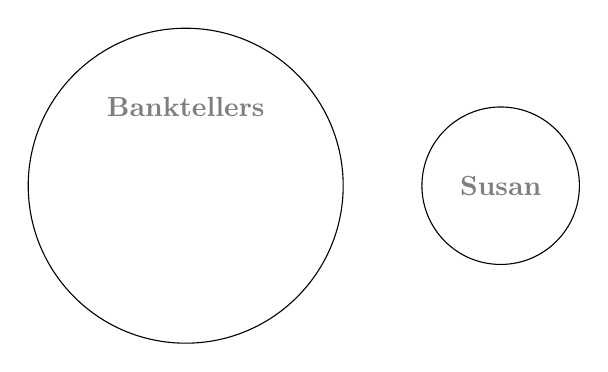
\begin{tikzpicture} 
    \begin{scope}[shift={(0cm,-2cm)}, fill opacity=0.5]
        \draw[fill=white, draw = black] (-1.5,0) circle (2);
        \draw[fill=white, draw = black] (2.5,0) circle (1);
    \node at (-1.5,1) (A) {\textbf{Banktellers}};
    \node at (2.5,0) (B) {\textbf{Susan}};
    \end{scope}
\end{tikzpicture} \\
\newline Susan is a bankteller, i.e Susan $\in$ Banktellers: \newline
\newline 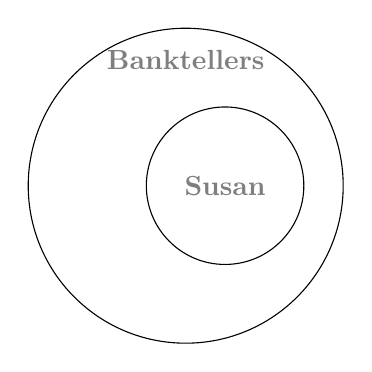
\begin{tikzpicture}
    \begin{scope}[shift={(0cm,-2cm)}, fill opacity=0.5]
        \draw[fill=white, draw = black] (-1.5,0) circle (2);
        \draw[fill=white, draw = black] (-1,0) circle (1);
    \node at (-1.5,1.6) (A) {\textbf{Banktellers}};
    \node at (-1,0) (B) {\textbf{Susan}};
    \end{scope}
\end{tikzpicture} \\


% \begin{venndiagram2sets}[
%        labelOnlyA={Susan},
%        labelOnlyB={2},]
%\end{venndiagram2sets}
